\linenumbers

\section{Feed-down subtraction}
%The methods for B feed-down subtraction
%As described in Sec.~\ref{sec:eff}, the prompt D meson production yields ${\rmd}N/{\rm d}\pt$ in Pb--Pb 
%collisions were obtained by subtracting the contribution of D mesons from B decays with the same procedure used for the measurement of the production cross sections in pp collisions~\cite{Acharya:2019mgn}. In detail, 

The feed-down contribution was estimated using 
the beauty production cross section from the FONLL calculation,
the B$\rightarrow$D decay kinematics are modeled with PYTHIA 8,
and the Monte Carlo efficiencies for feed-down D mesons. Thus, omitting for brevity the symbol of the $\pt$-dependence $(\pt)$, the fraction of prompt D mesons reads:
\begin{equation}
 \label{eq:fcNbMethod}
 \begin{split}
   f_{\rm prompt} &= 1-(N^{\rm D~feed-down~raw}/N^{\rm D~raw})\\
   &= 1 -  \left( \frac{{\rm d}^2 \sigma}{{\rm d}y \, {\rm d}\pt }
\right)^{{\sf FONLL}} _{{\rm feed-down}} \cdot
\frac{({\rm Acc}\times\epsilon)_{\rm feed-down}\cdot\Delta y \, \Delta\pt
\cdot {\rm BR} \cdot L_{\rm int}  }{ N^{\rm D~raw }  / 2} \, ,
 \end{split}
\end{equation}
where $({\rm Acc}\times\epsilon)_{{\rm feed-down}}$ is the 
acceptance-times-efficiency for feed-down D mesons and the factor 2 at the denominator
comes for counting both particle and antiparticle
are combined while in FONLL not. The variation of the parameters used for the FONLL B predictions is taken into account for the evaluation of the systematic uncertainties related to the feed-down D-meson subtraction. The fractions of prompt \Dstar , estimated via the $Nb$ method is performed by varying the parameters used in the FONLL B predictions, are shown in figure~\ref{fig:Dstarfeeddown_cent} and the systematic values are reported in~\ref{fig:Dstarfeeddown_cent2}.


 %are modeled with PYTHIA 8
%For Pb--Pb collisions, 
%the FONLL feed-down cross section in pp at $\sqrt{s}=5.02~\TeV$ 
%was scaled by the average nuclear overlap function $\langle \TAA \rangle$ in
%each centrality class.


%The systematic uncertainties on the prompt fraction of \Dstar -meson $f_{\rm prompt}$ , estimated via the $Nb$ method is performed by varying the parameters used in the FONLL B predictions, are shown in figure \ref{fig:Dstarfeeddown_cent}.

% The nuclear modification factor of the feed-down D mesons, $\RAA^{\rm feed-down}$,
%is related to the nuclear modification of beauty production in Pb--Pb 
%collisions, which is currently unknown. Taking advantage of the
%recent non-prompt J/$\Psi$ results from the CMS collaboration we
%assumed for the correction that the nuclear modification factor 
%for feed-down is equal to two times the one of the prompt D mesons ($\RAA^{\rm feed-down}=2\RAA^{\rm prompt}$) and varied this hypothesis
%in the range $1<\RAA^{\rm feed-down}/\RAA^{\rm prompt}<3$ ($1/3<\RAA^{\rm feed-down}/\RAA^{\rm prompt}<3$ for \Dsubs)
%to determine the systematic uncertainty. In the left panel of Fig. \ref{fig:Dsfeeddown010} (Fig. \ref{fig:Dsfeeddown3050})
%the variation of $\RAA^{\rm prompt}$ for \Dsubs mesons in the 0--10\% (30--50\%) centrality class is shown as a function of
%this hypothesis for some (all) $\pt$ intervals of the analysis. The resulting fraction of prompt \Dsubs in the same centrality class is reported in the right panel of the same figure.
%In Fig.~\ref{fig:Dzerofeeddown_cent} and \ref{fig:Dzerofeeddown_semicent} the variation of $\RAA^{\rm prompt}$ for \Dzero mesons in the 0--10\% and 30-50\% centrality classes are reported as a function of this hypothesis for some \pt intervals of the analysis in the left panel of each figure. The resulting fraction of prompt \Dzero in the same centrality classes are reported as line histogram in the right panel of the Fig.~\ref{fig:Dzerofeeddown_cent} and \ref{fig:Dzerofeeddown_semicent}.
%In addition, to estimate the systematic uncertainty, the perturbative uncertainty on the FONLL beauty production cross section was considered, by varying the b quark mass and the factorization and renormalization scales as suggested in~\cite{Acharya:2019mgn}. 

%======= Dstar =====
\begin{figure}[!b]
\begin{center}
 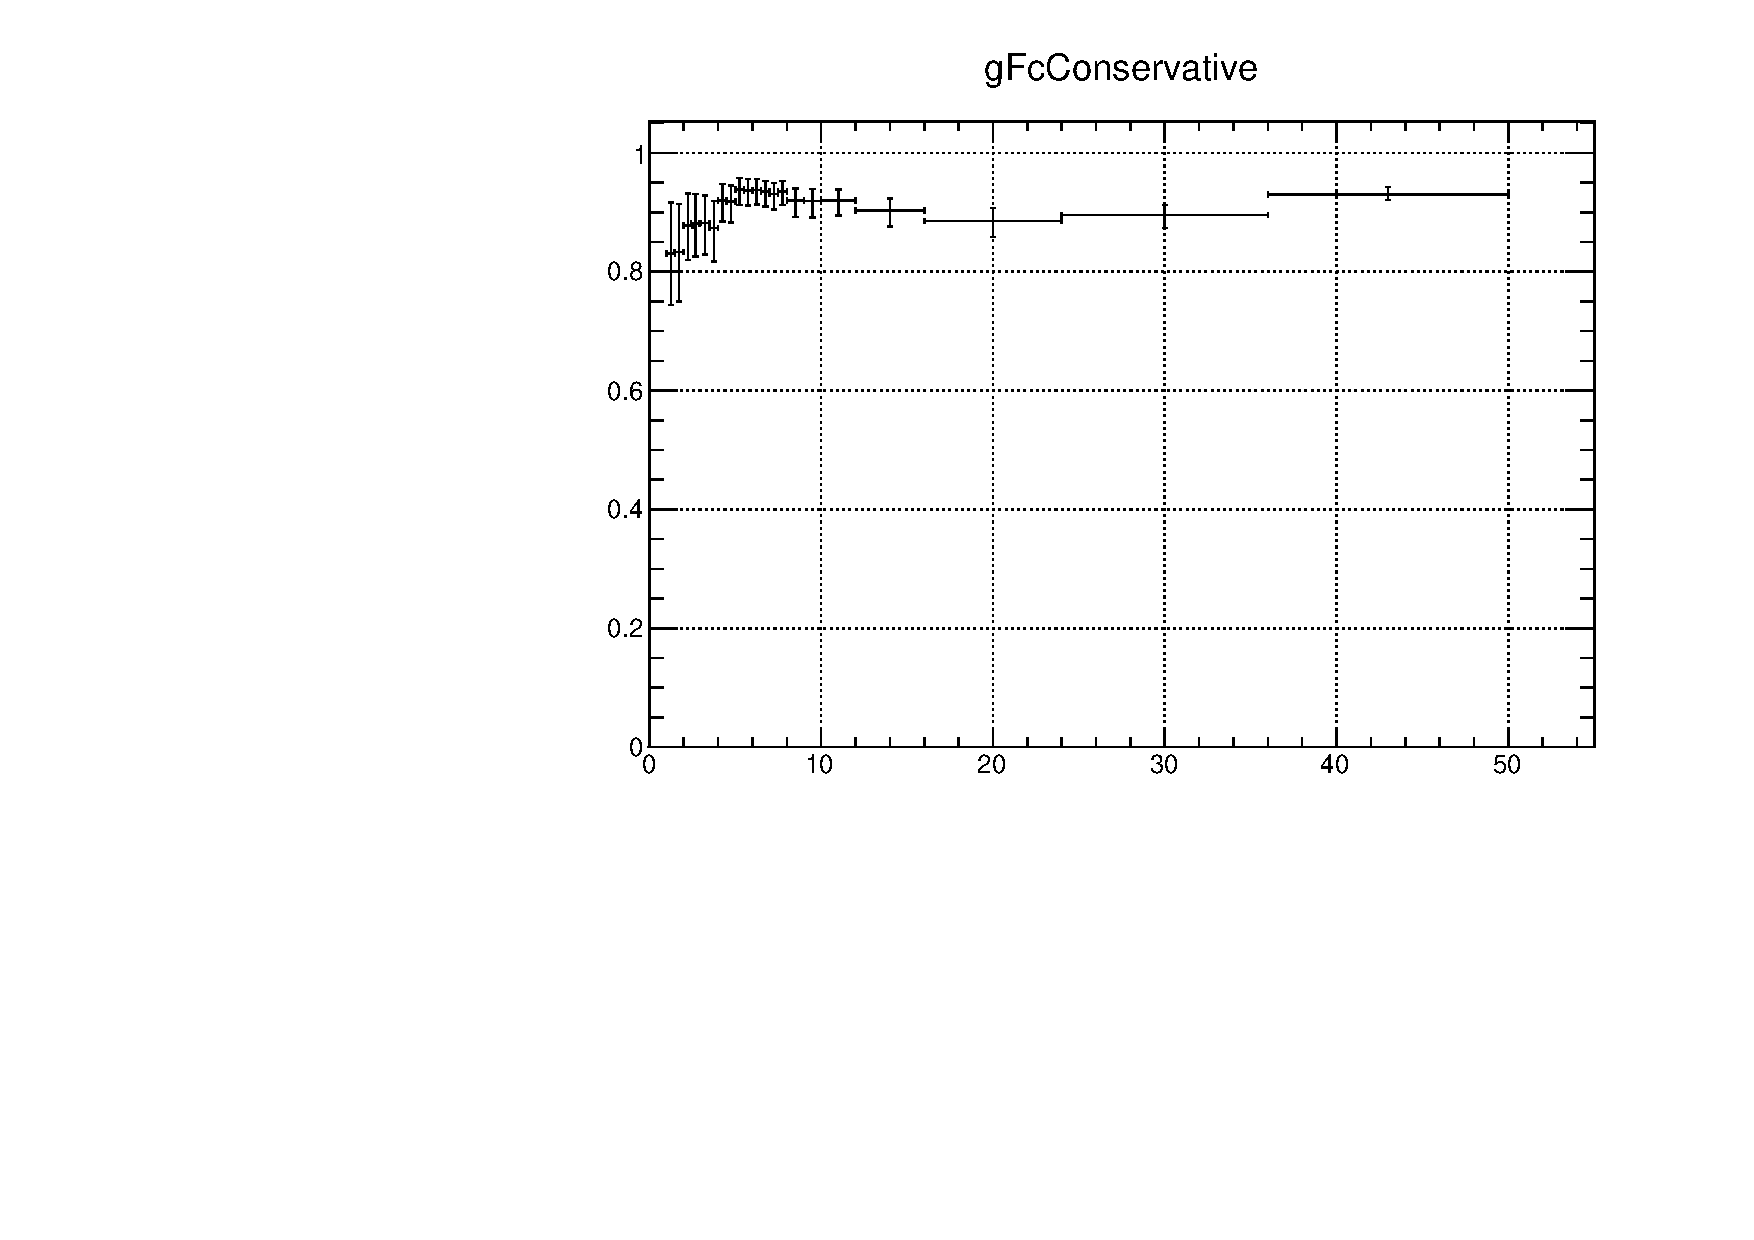
\includegraphics[width=0.85\textwidth]{figures/Dstar/pp13TeV/feed-down-syst-Dstar.pdf}
\caption{Fraction of prompt \Dstar estimated using the FONLL-based approach.}
\label{fig:Dstarfeeddown_cent}
\end{center}
\end{figure}

\begin{figure}[!b]
\begin{center}
 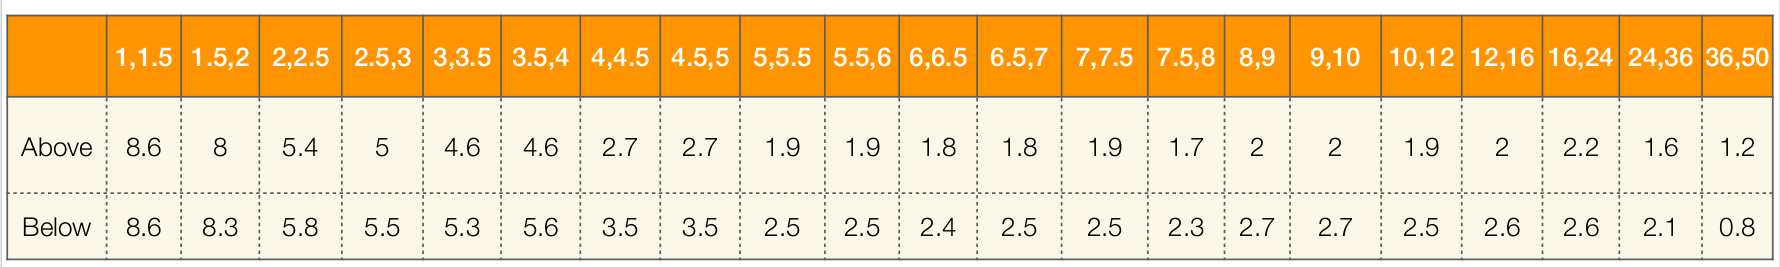
\includegraphics[width=1.0\textwidth]{figures/Dstar/pp13TeV/prompt-fraction.png}
\caption{Feed-down systematics.}
\label{fig:Dstarfeeddown_cent2}
\end{center}
\end{figure}
% prompt-fraction.png



